\documentclass[]{article}
\usepackage{lmodern}
\usepackage{amssymb,amsmath}
\usepackage{ifxetex,ifluatex}
\usepackage{fixltx2e} % provides \textsubscript
\ifnum 0\ifxetex 1\fi\ifluatex 1\fi=0 % if pdftex
  \usepackage[T1]{fontenc}
  \usepackage[utf8]{inputenc}
\else % if luatex or xelatex
  \ifxetex
    \usepackage{mathspec}
  \else
    \usepackage{fontspec}
  \fi
  \defaultfontfeatures{Ligatures=TeX,Scale=MatchLowercase}
\fi
% use upquote if available, for straight quotes in verbatim environments
\IfFileExists{upquote.sty}{\usepackage{upquote}}{}
% use microtype if available
\IfFileExists{microtype.sty}{%
\usepackage{microtype}
\UseMicrotypeSet[protrusion]{basicmath} % disable protrusion for tt fonts
}{}
\usepackage[margin=1in]{geometry}
\usepackage{hyperref}
\hypersetup{unicode=true,
            pdftitle={Group\_Proposal},
            pdfauthor={Team Fantasy},
            pdfborder={0 0 0},
            breaklinks=true}
\urlstyle{same}  % don't use monospace font for urls
\usepackage{graphicx,grffile}
\makeatletter
\def\maxwidth{\ifdim\Gin@nat@width>\linewidth\linewidth\else\Gin@nat@width\fi}
\def\maxheight{\ifdim\Gin@nat@height>\textheight\textheight\else\Gin@nat@height\fi}
\makeatother
% Scale images if necessary, so that they will not overflow the page
% margins by default, and it is still possible to overwrite the defaults
% using explicit options in \includegraphics[width, height, ...]{}
\setkeys{Gin}{width=\maxwidth,height=\maxheight,keepaspectratio}
\IfFileExists{parskip.sty}{%
\usepackage{parskip}
}{% else
\setlength{\parindent}{0pt}
\setlength{\parskip}{6pt plus 2pt minus 1pt}
}
\setlength{\emergencystretch}{3em}  % prevent overfull lines
\providecommand{\tightlist}{%
  \setlength{\itemsep}{0pt}\setlength{\parskip}{0pt}}
\setcounter{secnumdepth}{0}
% Redefines (sub)paragraphs to behave more like sections
\ifx\paragraph\undefined\else
\let\oldparagraph\paragraph
\renewcommand{\paragraph}[1]{\oldparagraph{#1}\mbox{}}
\fi
\ifx\subparagraph\undefined\else
\let\oldsubparagraph\subparagraph
\renewcommand{\subparagraph}[1]{\oldsubparagraph{#1}\mbox{}}
\fi

%%% Use protect on footnotes to avoid problems with footnotes in titles
\let\rmarkdownfootnote\footnote%
\def\footnote{\protect\rmarkdownfootnote}

%%% Change title format to be more compact
\usepackage{titling}

% Create subtitle command for use in maketitle
\newcommand{\subtitle}[1]{
  \posttitle{
    \begin{center}\large#1\end{center}
    }
}

\setlength{\droptitle}{-2em}
  \title{Group\_Proposal}
  \pretitle{\vspace{\droptitle}\centering\huge}
  \posttitle{\par}
  \author{Team Fantasy}
  \preauthor{\centering\large\emph}
  \postauthor{\par}
  \predate{\centering\large\emph}
  \postdate{\par}
  \date{4/12/2018}


\begin{document}
\maketitle

\subsubsection{Introduction}\label{introduction}

Fantasy sports have been a popular way for fans to get more
knowledgeable and interested into the sports they love. Fantasy sports
began as board and card games 50 years ago and have exploded since it
was introduced to the internet. The appeal to fantasy sports is they
allow fans to act as owners, managers and coaches of professional teams
by allowing them to draft a team and watch the season unfold
successfully or catastrophically.

One of the most popular fantasy sports people participate in is fantasy
basketball for the NBA. The first step when participating in fantasy
basketball is drafting a team which usually consists of about thirteen
players and there can be restrictions on how many players of each
position an individual may draft (This all depends on the specific
league one participates in). Once a team has been drafted, the league
determines which statistics will be counted as fantasy points and how
many fantasy points each statistic is worth. For example, a block counts
for 1 fantasy points while a steal counts for 2. After this has been set
and the NBA season begins, each night the fantasy points for each
participant is totaled and the participant at the end of the regular
season with the most fantasy points wins. Therefore, when drafting
players one needs to be able to analyze players pasts statistics,
predict future player statistics and weigh them based on the determine
fantasy point scoring system to draft a team that will make them the
optimal amount of points for the season.

With all the possible statistics to consider (depending on the
particular fantasy league one is apart off), we hope to create a tool
for fantasy NBA participants to use during their draft to help them make
the best possible team selections. This tool ideally would allow a
participant to input their individual league scoring system and the
players that have already been selected in the draft and return the best
possible team they could select based on NBA players statistics in the
past five years and predictive modeling. Along with the output of the
predicted best team, there will be graphical representations of why the
particular players were chosen.

Our idea stated above matches the course focus on statistical programing
because it involves taking a large data set and using a data pipeline in
order to use that dataset to make prediction on NBA players future
performance based on their past performance (their past statistics). We
will also be providing visual representation of the data in the form of
graphs which will compare players, as well as, coding a shiny app for
fantasy league participants to easily customize the data pipeline to
their personal fantasy league rules.

\subsubsection{Related Work}\label{related-work}

Someone had tried to analyze the data to prepare for the draft strategy
for the new season in 14-team basketball league. He took the data from
cutting and copying on ESPN.com and NBA.com. He put a flat file of the
top 250 players from the previous season. Then he created a binary
variable for the top 42 players (3 players per 14 teams). The ``1''
means the player is a top 3 players, otherwise he is not. He used 28
independent variables from the previous season to identify the ``top 42
players''. He came up with conclusions that field-goal percentage,
assist and blocks are the difference-makers because most players in NBA
are good at points and rebounds. However, assists and blocks are rarer
so that they are more valuable to a fantasy team. Other projects include
computing the average stats for each categories of players. Some of the
other are having the graph comparing the specific player and league's
average. Or group comes up data calculating the standard deviation to
see how far away a player is from average.

Comparing to other projects, our group will use the bigger dataset. Most
projects are using previous year's dataset for predicting the future
data. We are going to use the data in the past five years to make a more
precise prediction for player's future performance. One of the most
difference is that our group will use the Shiny app in R. Most projects
online are only included complex graphs or prolix passages that make
reader hard to understand their ideas. For us, we will make the Shiny
app that looks very easy and clear for people to manipulate. For
example, we will list all our players. People can click each of them.
Then they can look at each player's trend data whether they are getting
better or worse or the graph comparison between players. It is very
simple for people to control in the app. All the data fantasy NBA
participants want it will exist in the app. If they want to see the
difference between players, they also can click the graphs to see their
difference in various categories, such as points, rebounds, assists and
so on, so they will figure out what type of player they are looking for.
Thus, our app is serving as a recommender for fantasy basketball player
to select their team.

\subsubsection{Methods}\label{methods}

The methodology for our group project will closely follow the analytical
data pipelines phases. As we need to import data related to basketball
players off the internet we will need to use SelectorGadget as well as
the rvest package to scrape this information offline. We plan to import
the data from \url{http://www.basketball-reference.com} assuming that we
have continued success in scraping from that site. Then we will have to
tidy the data, so it is likely we will need stringr, rvest, and tidyr.

Our goal in tidying the data is to have the data organized so that each
player's average score during a year in the NBA is an observation. So,
for every year a player has played in the NBA they would have an extra
observation. Each observation would contain the name, organization,
position, and age of the player. Along with these three factor variables
and one-time variable, likely an integer, we will have statistics
variables for the average of the season, likely some form of numeric.
The desired statistics follow the most widely used statistics in fantasy
NBA under the point-based scoring method, where each statistical
category counts for a set number of points. The categories likely to be
used are points, rebounds, assists, offensive blocks, defensive blocks,
steals, fouls, turnovers, field goal percentage, and free throw
percentage.

How we plan to model our NBA league will directly impact how we
transform the data, so it must be discussed. NBA fantasy can be done
many ways, but the way we are going to be analyzing is based on the
fantasy points method of NBA fantasy. In this method the group playing
sets each statistic to have a point value and the points for your
fantasy team are calculated real time. At the end of the season those
with more points win. This model seemed the most straight forward in
implementing our project. It will also allow for a large amount of user
customization when the project is done, as a group of friends can decide
how many points each statistic is worth, or if they are worth none.

Then we must transform the data of into some sort of prediction for the
coming years data. This part can be done through time series modeling.
We would take every individual player individual statistics and use a
time series model to predict how they will perform in that statistic
next year. Now we have a new transformed data for each player containing
predictions for their average statistics per game next year. We would
then allow for user input to give statistics more weight in totaling
points. So, the final dataset that we show is our prediction data set
multiplied by a vector of user weight inputs, as well as former years
averages multiplied by user inputs.

The visualization part concerns how we display this information in
graphs, as well as how we display the entire shiny application. At this
moment the overall layout for our shiny app consists of a tab for
changing settings on one side, a tab for picking players on the other
side, and a list of picked players for each team on the bottom. On the
side with players we will have rows sorted by players expected total
score next year, highest first. These players will descend the page,
each player taking up a row. On the players will be a summary of who
they are, along with the current years statistics and our predicted
statistics. Next to these numbers will be a button that switches to
graphs pertaining to this player. By clicking on multiple boxes, we can
see different player comparisons.

Regarding the graphs that we will compose using our data, the graphs are
either comparative between players, or analyzing an individual player
over time. When comparing players, we will use side by side bar plots
with the x axis being source of points and the y axis being amount of
points. The bars will be sorted by individual statistic, points with
points and assists with assists. This allows direct comparison between
the two chosen players to determine who is better at what category, as
well as who is better. When analyzing an individual player change
throughout time we will use a scatterplot graph with years on the x axis
and total points on the y axis. This scatterplot will be accompanied by
a best fit regression line to be determined while analyzing the data,
although we suspect it to be parabolic with players getting worse with
age after they peak. Along with normal points from actual years we will
highlight our predicted point, which is the point that our best fit line
intersects with next year. We could also implement it where if a user
clicks on a predicted or past point they can see a summary of what
statistics a player specializes in during any year.

In summation we will have to write code that retrieves the data for
current players as well as these players former years. We then must
write code that sorts this data into tidy and usable datasets. Then we
need to write a time series model that takes players past NBA
performances and predicts next years performance. We then must code a
shiny interface that takes these predicted and historic point values and
displays them along with players name, team, and position. Lastly, our
shiny application must have a way to create graphs that explain
different players differences as well as the idea behind our prediction.

\subsubsection{Feasibility}\label{feasibility}

We believe that all the goals for this fantasy team selector tool we
will be able to create by the end of the semester. This includes the
graphical representations of players current and past statistics,
graphical comparisons of players, a shiny app that allows for
customizability to different league rules and the selection of a fantasy
league team. However, if we do run into complications during the
creation process, we may have to scale back the amount of
customizability provided in the app in order to complete this project on
time.

In order to complete the project, we must complete the following
tasks\ldots{}

\begin{enumerate}
\def\labelenumi{\arabic{enumi}.}
\item
  Web scrape and tidy the NBA statistics data (Anne)
\item
  Write code to create prediction data through time series modeling
  (Conrad)
\item
  Visually/Graphically represent the prediction data (Zhaobin)
\item
  Create the shiny app (Everyone)
\end{enumerate}

\begin{figure}
\centering
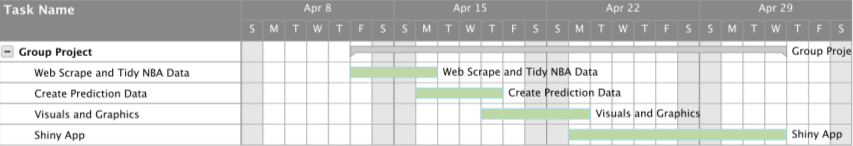
\includegraphics{ganett_chart.png}
\caption{Figure 1. The ganett chart above describes the timeline set in
place to complete the tasks stated for this project.}
\end{figure}

\subsubsection{Conclusion}\label{conclusion}

In general, our goal is to help fantasy basketball fans draft their
players by analyzing players' past statistics in order to make the
optimal team for themselves. We will create the tool for fantasy NBA
participants who will use it during the draft to come out the best team
selections. Inside the app, we will follow the analytical data pipelines
phases. We are going to import data from website, and then we will tidy
the data by using stringr, rvest, and tidyr. For the dataset, we will
organize each player's average score. Each observation will contain the
name, team name, position, weight, age, and so on. The scores will come
out by the algorithm of fantasy inside, likely each statistical category
counts for a set number of points. The variable include points,
rebounds, assists, blocks, steals, turnovers, field goal percentage, and
free throw percentage. We will also be using the data to predict for the
coming years data by time series modeling. The method is to take every
individual player' statistics to a use series model, so we can predict
how individuals will perform next year. After that, the user will be
able to see the prediction data set multiplied by a vector of user
weight inputs. Inside the App, we will also include the visualization
part. The overall layout for shiny app will consist a tab for changing
setting on one side. There is another tab for clicking players on the
other side. There will be a list of selected players on the bottom.
Inside the player click, we will have rows sorted by players expected
total score in upcoming year in descending order. In each player's page,
we will include some graphs. For the graphs, we will compare players and
analyze individual player over time. For comparing players, will be
using side by side bar plots that the x-axis represents points and
y-axis represents the transferred fantasy points. It will be sorted by
many categories of statistics, such as points, rebounds, assists, and so
on. We will be able to see directly who is better according to the
graphs. For the individual player graph, we will be using a scatterplot
graph with years on the x-axis and the total fantasy points on the
y-axis. It will be presented by the best fit regression line to be
determined. Again, our fantasy team selector tool will include the
graphical representations of current and past statistics of players and
graphical comparisons of players. By looking at some pre-existing
projects, I find out that out project's novelty is the convenience and
clear path to the success of the fantasy NBA life. Some articles are
being too long or complex analysis of basketball itself. Others are
having no graphs or comparisons between players. Our app will help
people tidy the data so that they can click whatever player they want to
look at inside the app. What is more, when they have trouble at deciding
to select player, they can open the charts or comparison graphs to see
what kind of categories they need to. Overall, I think it will be a
great tool for fantasy NBA participants to use.

\subsubsection{References}\label{references}

Davis, Nickolas W., and Margaret Carlisle Duncan. ``Sports Knowledge Is
Power Reinforcing Masculine Privilege Through Fantasy Sport League
Participation.'' Journal of Sports and Social Issues 30, no. 3 (August
1, 2006): 244-46.

Hadley Wickham, Romain Francois, Lionel Henry and Kirill Müller (2017).
dplyr: A Grammar of Data Manipulation. R package version 0.7.4.
\url{https://CRAN.R-project.org/package=dplyr}

H. Wickham. ggplot2: Elegant Graphics for Data Analysis. Springer-Verlag
New York, 2009.

Hadley Wickham (2016). rvest: Easily Harvest (Scrape) Web Pages. R
package version 0.3.2. \url{https://CRAN.R-project.org/package=rvest}

Hadley Wickham (2018). stringr: Simple, Consistent Wrappers for Common
String Operations. R package version 1.3.0.
\url{https://CRAN.R-project.org/package=stringr}

Hadley Wickham and Lionel Henry (2018). tidyr: Easily Tidy Data with
`spread()' and `gather()' Functions. R package version 0.8.0.
\url{https://CRAN.R-project.org/package=tidyr}

Raney, Arthur A., and Jennings Bryant. 2014. Handbook of Sports and
Media. New York, New York: Routledge, Taylor \& Francis Group.

Stefan Milton Bache and Hadley Wickham (2014). magrittr: A Forward-Pipe
Operator for R. R package version 1.5.
\url{https://CRAN.R-project.org/package=magrittr}

Winston Chang, Joe Cheng, JJ Allaire, Yihui Xie and Jonathan McPherson
(2017). shiny: Web Application Framework for R. R package version 1.0.5.
\url{https://CRAN.R-project.org/package=shiny}

Wrinn, Corey. 2015. ``Data Analysis in Fantasy Basketball: Making it
Easy to Beat Your Friends.'' Rapidinsightinc.com. Oct.22, 2015.
\url{http://www.rapidinsightinc.com/data-analysis-fantasy-basketball-making-easy-beat-friends/}

Tang, Steven. 2014. ``Drafting a Fantasy Basketball Team With Help From
Statistics and a Knapsack.'' Medium.com. Oct 21,2014.
\url{https://medium.com/fun-with-data-and-stats/drafting-a-fantasy-basketball-team-c94967464908}

\subsubsection{Appendix}\label{appendix}

\section{Variable List}\label{variable-list}

Data is organized in two different ways, by year with each player having
6 observations, or by player, with each player having one observation.
The data that is organized by player is split into multiple data sets by
player position. All data sets mentioned are in the folder
Fantasy\_Basketball

Varialbles in the data set organized by player

X1: A number representing the players position in an aplphabetically
organized list Name: Player's name, one for each player Age: Players Age
in year 2018 Position: Players Position


\end{document}
